\documentclass[letterpaper,twocolumn,10pt]{article}
\usepackage{usenix,epsfig,endnotes}

%%%%%%%%%%%%%%%%%%%%%%%%%%%%% DELETE AFTER %%%%%%%%%%%%%%%%%%%%%%%%%%%%%%%%%%%%
\usepackage{lipsum}
\usepackage{xargs}                      % Use more than one optional parameter in a new commands
\usepackage[pdftex,dvipsnames]{xcolor}
\usepackage[colorinlistoftodos,prependcaption,textsize=tiny]{todonotes}
\newcommandx{\unsure}[2][1=]{\todo[linecolor=red,backgroundcolor=red!25,bordercolor=red,#1]{#2}}
\newcommandx{\change}[2][1=]{\todo[linecolor=blue,backgroundcolor=blue!25,bordercolor=blue,#1]{#2}}
\newcommandx{\info}[2][1=]{\todo[linecolor=OliveGreen,backgroundcolor=OliveGreen!25,bordercolor=OliveGreen,#1]{#2}}
\newcommandx{\improvement}[2][1=]{\todo[linecolor=Plum,backgroundcolor=Plum!25,bordercolor=Plum,#1]{#2}}
\newcommandx{\thiswillnotshow}[2][1=]{\todo[disable,#1]{#2}}
\setlength{\marginparwidth}{2cm}
\usepackage{xcolor}
\newcommand{\note}[1]{\noindent{\color{red}\textbf{#1}}}
\definecolor{jazzberryjam}{rgb}{0.65, 0.04, 0.37}
\definecolor{ultramarine}{rgb}{0.07, 0.04, 0.56}
\newcommand{\notegp}[1]{\note{\color{jazzberryjam}[\textsc{Guillaume:} #1]}}
\newcommand{\noteaa}[1]{\note{\color{ultramarine}[\textsc{Arif:} #1]}}

%%%%%%%%%%%%%%%%%%%%%%%%%%%%%%%%%%%%%%%%%%%%%%%%%%%%%%%%%%%%%%%%%%%%%%%%%%%%%%%%
\usepackage[none]{hyphenat}
\let\origref\ref
\def\ref#1{\textbf{\origref{#1}}}
\usepackage{multirow}
\usepackage{rotating}
\usepackage{url}
\usepackage{hyperref}

\clubpenalty=10000 \widowpenalty=10000 \displaywidowpenalty=10000



%%%%%%%%%%%%%%%%%%%%%%%%%%%%%%%%%%%%%%%%%%%%%%%%BEGIN%%%%%%%%%%%%%%%%%%%%%%%%%%%%%%%%%%%%%%%
\begin{document}

%don't want date printed
\date{}
\title{\Large \bf Towards Fog-Aware Kubernetes}
\author{
{\rm Ali J. Fahs}\\
Univ Rennes, Inria, CNRS, IRISA\\
ali.fahs@irisa.fr
\and
{\rm Guillaume Pierre}\\
Univ Rennes, Inria, CNRS, IRISA\\
guillaume.pierre@irisa.fr
}
\maketitle
\thispagestyle{empty}


\subsection*{Abstract}

Kubernetes is a mature and lightweight container management platform
that easily scales to large-size clusters. However, we argue that in
its current form it is essentially location-unaware, which makes it
unsuitable to handle fog computing workloads. We therefore propose a
roadmap of extensions to fill the gap between Kubernetes and the fog.

%%%%%%%%%%%%%%%%%%%%%%%%%%%%%%%%%%%%%%%%%%%%%%%%%%%%%%%%%%% INTRODUCTION %%%%%%%%%%%%%%%%%%%%%%%%%%%%%%%%%%%%%%%%%%%%%%%%%%%
\section{Introduction}
%The introduction of Fog computing. DONE

Fog computing extends the concept of cloud computing with additional
resources which are organized in a very different manner: when cloud
platforms aim to concentrate huge amounts of computing resources in a
small number of data centers, fog computing rather aims to distribute
resources as broadly as possible across some defined area so some
resources are always located in the immediate vicinity of every end
user's devices. Proximity between end user devices and the fog
computing resources serving them is essential for application which
require ultra-low network latencies (e.g., augmented reality
applications) or where it is desirable to process data where input
data was produced and processing results will be used (e.g., IoT data
analytics).


% \hskip .7em In a world where centralized data centres have been proven to be cost-effective, the big players of cloud services are relaying on few data centres to serve millions of users all over the globe. 

% Such a model have seen the light due to the lack of interest in locating the services in a specific geolocation. The location of the data centres are chosen according to some factors like power cost, disregarding the impact on the end-to-end latency of the service. Furthermore, the cloud service user is not informed about the location of the server, where this location awareness is sometimes vital for specific types of application {\em (e.g., IoT applications)}.

%The separation was not limited to the management alone, but also to the geographical location. 

An essential requirement for a fog computing platform is therefore to
take the location of fog resources and end-user devices into account
to ensure proximity between the two. However, most platforms available
today such as OpenStack, Docker Swarm, Mesos and Kubernetes were
initially designed with datacenter deployments in mind and therefore
often do not provide location awareness in their resource scheduling
and/or load balancing algorithms.



% Nowadays, some applications require lower latencies and location awareness. These requirments will be provided by an extended paradigm of cloud computing called fog computing\cite{bonomi2011connected,Bonomi:2012:FCR:2342509.2342513}.

% %The resource Fog provide.
% The fog computing architecture included an intermediary level between the end devices and the cloud computing data centres. This platform provides compute, storage and networking resources, similar to clouds. Yet, the difference lies in the proximity to the user, low latency, distribution, and location awareness. 

% %Fog targeted application and user proximity.
% Unlike clouds, which relies on a handful of gigantic data centres, fog is based on the idea of spreading several points of presence in the proximity of the user. Since the end devices are close to the source, the latency can be significantly reduced, which will improve the users' experience. All of this can be done while considering the location of the access point as an important measure of the workload scheduling.

%Platforms for fog.
% Since the concept of fog is relatively new, no platform was designed to assist fog architecture. However, a fog computing cluster can be deployed on top of cloud platforms like Docker swarm, Mesos, and Kubernetes. Out of these platforms we have chosen Kubernetes to be tested and improved for the reasons that will be discussed in the paper.

In this paper we focus on understanding and addressing the limitations
of Kubernetes in a fog computing scenario. Kubernetes matches many of
the requirements of a fog platform in that it is highly scalable, it
can run even on very limited machines thanks to its usage of
lightweight containers rather than VMs. It is also a very open and
mature platform which is now familiar to a large community of
application developers. We discuss the limitations of the current
implementation and propose a roadmap of the different improvements
that remain necessary to make Kubernetes an equally attractive
platform for fog computing scenarios as it is for cloud computing
scenarios.

%Why Kubernetes is not compatible with Fog computing (briefly).
% Although Kubernetes provide automation, still it doesn't have all the features to full-fill the definition of the fog.    

% %paper objective 
% In this paper, we contribute by demonstrating our vision through a roadmap of the steps that should be taken to achieve fog-aware Kubernetes.


%Explain organization of the report, what is included, and what is not.
This paper is organised as follows. In Section~\ref{sec:plat}, we
briefly acknowledge the possible fog computing platforms. In
Section~\ref{sec:kube}, we introduce Kubernetes as a platform, discuss
the advantage and disadvantages in the context of fog. In
Section~\ref{sec:road}, we suggest the next steps through a
roadmap. Finally, in Section~\ref{sec:conclusion} we conclude.


%%%%%%%%%%%%%%%%%%%%%%%%%%%%%%%%%%%%%%%%%%%%%%%%%%%%%%%%%%% Fog Computing %%%%%%%%%%%%%%%%%%%%%%%%%%%%%%%%%%%%%%%%%%%%%%%%%%%
\section{State of the art}\label{sec:plat}

A fog computing platform is in charge of managing compute, storage and
networking resources that are physically distributed across a
geographical area such as a building, a neighborhood and a
city~\cite{Bonomi:2012:FCR:2342509.2342513, fogecosystem}. It relies
on virtualization techniques to support many independent end users and
applications making use of these resources. For ressource-efficiency
reasons we focused our efforts on platforms which rely on lightweight
container technologies rather than virtual machines, enabling us to
envisage fog computing platforms making use of resources as limited as
Rasperry PIs for example~\cite{vankempen:hal-01446483}.


% architecture necessarily includes a number of
% infrastructure management tools such as a scheduler, fault tolerance,
% orchestration. In our search for a proper platform we have focused on
% the ones that support containers, for the lightness and portability
% containers offer over Virtual Machines.

OpenStack++ is a set of OpenStack extensions that implements
cloudlets: small-scale cloud data centers that are dispersed at the
edge of the Internet~\cite{openstackplusplus}. A set of cloudlets may
arguably be used to implement a fog platform. However, OpenStack++
bases itself on VM technologies, which does not match our requirements
for resource efficiency in the presence of large numbers of
independent applications sharing the resources of modest computing
devices.

PiCasso~\cite{picasso} is a container orchestration platform that
specifically targets edge clouds with a focus on lightness and
platform automation. However, it is still under development and not
publicly available.

The most prominent container orchestration engines are Docker
Swarm~\cite{swarm}, Apache Mesos~\cite{mesos} and
Kubernetes~\cite{burns2016borg}, which all provide advanced features
for container scheduling, cluster management, and support for
large-scale clusters~\cite{kub-vs-swarm}. They are currently the most
mature systems to support the deployment of a fog/cloud
platform. However, they lack a number of functionalities that are
essential for large-scale fog computing scenarios, as we discuss in
the next section in the specific case of Kubernetes.

  
%%%%%%%%%%%%%%%%%%%%%%%%%%%%%%%%%%%%%%%%%%%%%%%%%%%%%%%%%%% Kubernetes %%%%%%%%%%%%%%%%%%%%%%%%%%%%%%%%%%%%%%%%%%%%%%%%%%%
\section{Kubernetes and Fog Computing}\label{sec:kube}

We have chosen to base our efforts on Kubernetes.  In particular, it
offers many functionalities such as the concepts of pods and services,
auto-scaling, and a clean separation between the applications and the
underlying platform. It has also attracted a very large community of
users and developers which position it as a highly mature platform.

However, Kubernetes was designed with cloud computing scenarios in
mind. We briefly present its main architecture, and discuss its
strengths and current limitations when trying to use it as the basis
of a fog computing platform.



\subsection{Kubernetes Architecture}

\begin{figure}[t]
  \centering
  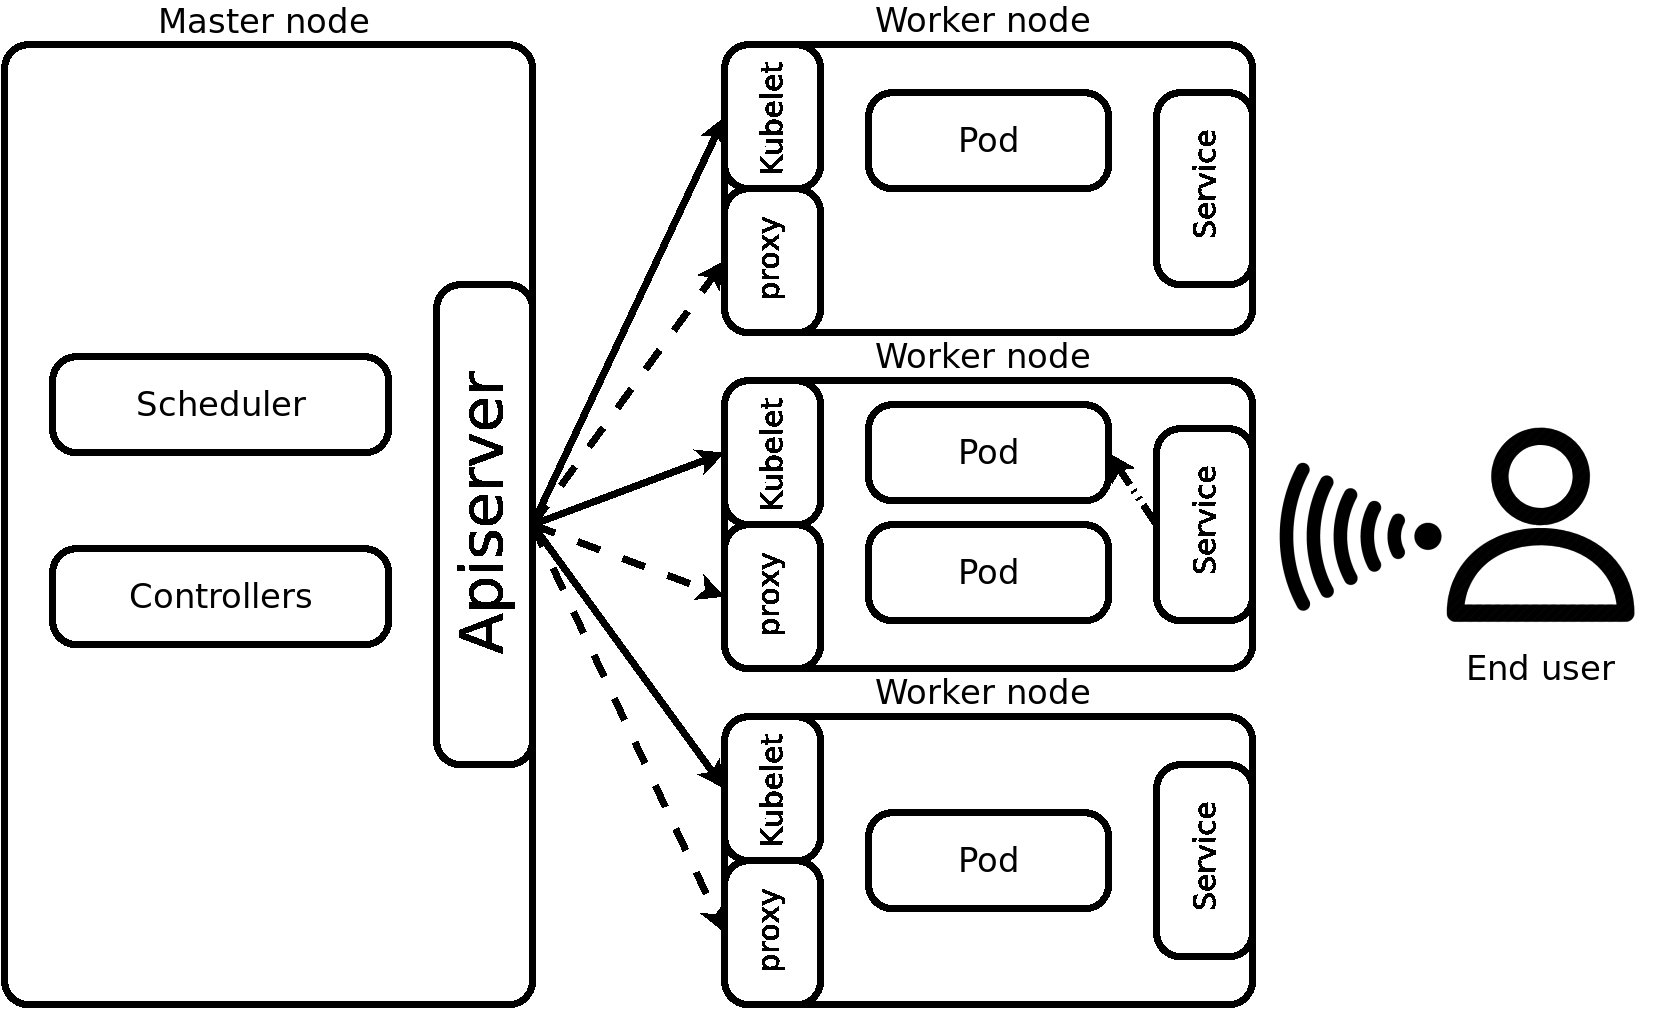
\includegraphics[width=\linewidth]{images/arch.png}
  \caption{Kubernetes architecture} 
  \label{fig:arch}
\end{figure}

%paragraph linking
Kubernetes is an open-source container-based platform which can manage
the deployment and orchestration of service instances over a
large-scale computing infrastructure. As presented in
Figure~\ref{fig:arch}, Kubernetes cluster consist of one master node
and multiple worker nodes. The master node is responsible for
monitoring and managing the cluster via a variety of control
components such as the resource scheduler and the deployment
controllers. Conversely, the worker nodes actually execute user
applications inside containers according to instructions given by the
master node.

Kubernetes organizes containers in the form of \emph{Pods}, where a
pod is a tight group of logically-related containers running in a
single worker node. Containers which belong to a single pod can
communicate with each other using an isolated private network. Pods
are not usually managed directly by the users. Rather, users are
expected to create a \emph{Deployment Controller}, which is in charge
of the creation and management of one or more identical pods providing
the expected service. Such a set of pods can be made publicly
accessible from external end users by creating a \emph{Service} which
acts as a frontend for the group of pods.

The master may schedule each pod in any worker node, by default chosen
as the worker node with the lowest load in the system. Since pods may
be placed in different nodes, communication is established as follows:

\begin{itemize}
\item Container-to-container communication within a pod is enabled
  using the Container Network
  Interface\footnote{\url{https://github.com/containernetworking/cni}},
  which enables connectivity between containers within a single
  machine.
\item Communication between the pods is ensured a component called
  \emph{kube-proxy} which relies on \emph{iptables} to establish the
  appropriate routes.
\end{itemize}

\begin{figure}[t]
  \centering
  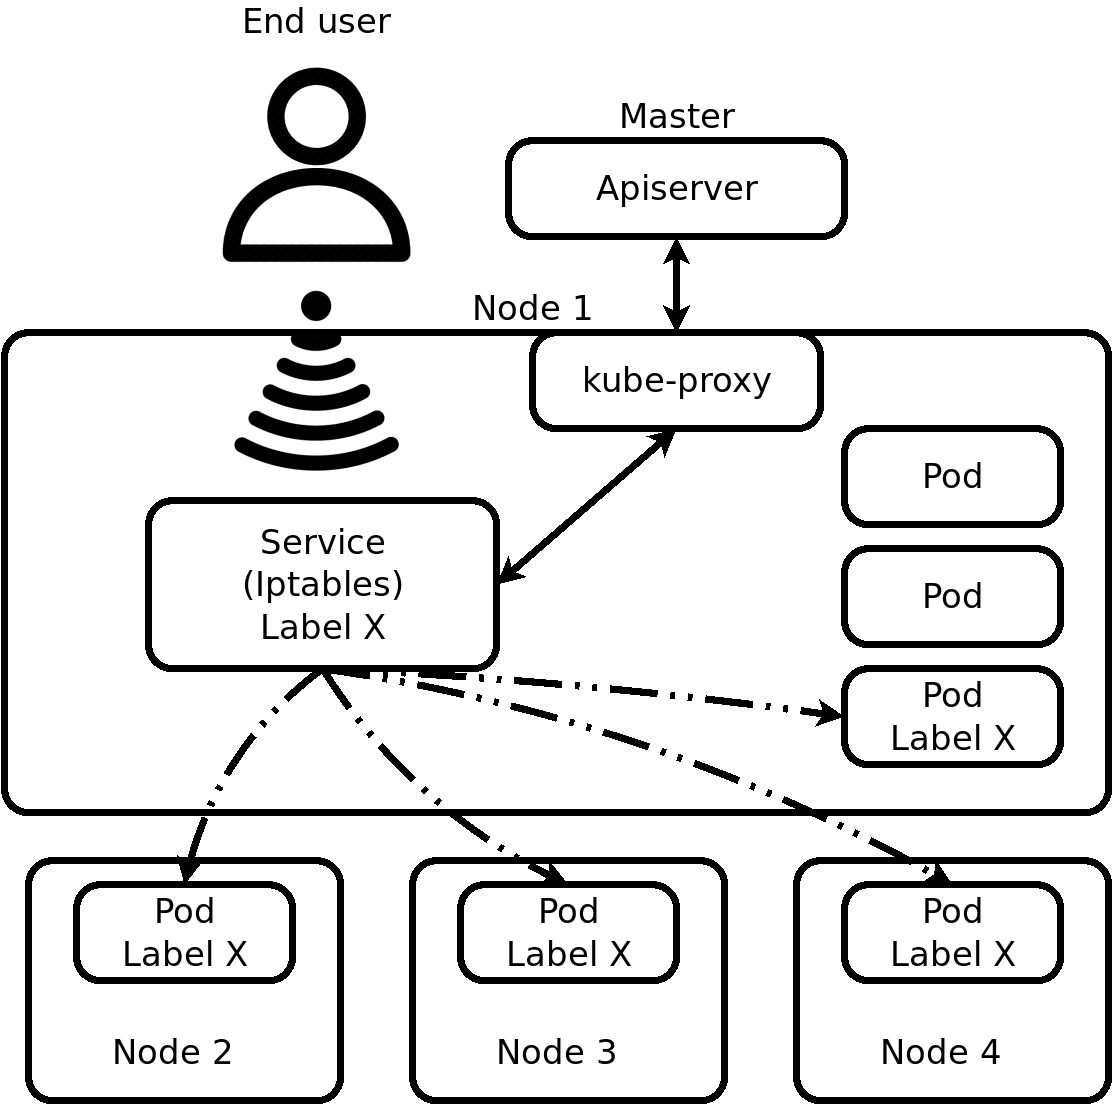
\includegraphics[width=.9\linewidth]{images/svc.png}
  \caption{Organization of a Kubernetes service}
  \label{fig:svc}
\end{figure}

As illustrated in Figure~\ref{fig:svc}, the main purpose of a
Kubernetes service is to connect end users to the exposed
pods. Whenever a pod is exposed, it takes a virtual IP address (called
endpoint) and receives a label (Label X in the figure). The Service
then acts as a load balancer between all the registered pods with the
chosen label. The selection of the pod an end user request gets
redirected to a load-balancing policy such as round-robin, source
hashing, and shortest expected delay.

\medskip In the next sections we discuss the strengths and weaknesses
of this architecture in the specific case where one chooses to use
Kubernetes as the basis for a fog computing platforms.


\subsection{Kubernetes Advantages}

Kubernetes has a number of properties that make it a great platform in
cloud as well as fog computing environments.


\begin{description}
\item[Scalability.] A fog architecture relies on wide distribution of
  marge numbers of points of presence, spread over a potentially large
  geographical area. Kubernetes supports large-scale clusters up to
  5000 nodes and 150,000 pods, which largely matches the scalability
  requirements of most fog computing scenarios.

\item[Simple management.] Managing a Kubernetes cluster is very simple
  and robust. For example, adding new nodes is as simple as running a
  join command, and the master node will take care of everything,
  without the need of manual intervention.

\item[Containerization.] Running applications inside containers is the
  new trend over virtualization. Containerization outperform
  virtualization in lightness and in the facilitation of application
  packaging, shipping, and deployment. This the reason why cloud
  platforms like Kubernetes are built around this concept, where the
  benefits of containers also applies in fog computing architecture.

\item[Deployment.] Kuberentes deployment is done using deployment
  controllers located in the master node, these controllers receives
  user's request for new deployments and interpret them in terms of
  pods. The user will monitor the pods as a deployment, and any
  failure of a pod or a node would be automatically resolved without a
  manual intervention.

\item[Community.] Kubernetes is surrounded by a large-scale community
  consists of thousands of contributors from the industrial and
  research field, meeting and events, and forms to file issues and ask
  questions.  The support provided by this community eases the
  development of the software for everyone, where a number of features
  Kubernetes have today were developed by this community.
\end{description}


\subsection{Kubernetes Disadvantages}

\begin{description}
\item[Centralization.]  K8's cluster is composed of master node and
  worker nodes, all the decision of the cluster are made by the
  master, and all the cluster controllers are located there. This
  imposes higher latencies when executing jobs like deploying a
  container, also heavy computations are done in the master node to
  take all the decision of the cluster.\change{rephrase!}

\item[Location awareness.]  The fact that K8's does not support
  location awareness is not shocking, since K8's is a cloud
  platform. Yet the location awareness is the number one
  characteristic of fog
  computing~\cite{Bonomi:2012:FCR:2342509.2342513}.  The
  characteristic of location awareness is mainly required to allow the
  fog to trace the closest available resource, which will improve the
  latency.

\item[Load balancing.]  Load balancing in Kubernetes is limited to
  external load balancers used in the cloud providers, since the fog
  is definitely not built in the cloud provider hardware then now load
  balancing options are not available for the fog.\unsure{need to
    check more}

\item[Scheduling regardless the location.] Neither the deployment of
  the containers, nor the scheduling of the incoming requests from the
  application users is related to the location of the node. As a
  result we will end up by the jobs traversing more hops in the
  network before reaching the targeted nodes, which implies higher
  end-to-end latencies.\change{rephrase!}


\end{description}

%%%%%%%%%%%%%%%%%%%%%%%%%%%%%%%%%%%%%%%%%%%%%%%%%%%%%%%%%%% Roadmap %%%%%%%%%%%%%%%%%%%%%%%%%%%%%%%%%%%%%%%%%%%%%%%%%%%
\section{A Roadmap Towards Fog-aware Kubernetes}\label{sec:road}

Achieving a platform that full-fill the requirements of the fog depend on achieving two main things: a low latency that will support the latency sensitive applications, and a platform that consider resource's location when making scheduling decisions. In the previous section, we have explained how K8's lack those two pillars, however enhancing K8's to support them is achievable.

Kubernetes code\endnote{https://github.com/kubernetes/kubernetes} was configured on a cluster made up of 4 Raspberry Pi's(RPi's), one of the RPi acts as the master node and the others are worker nodes. In kubernetes, we have looked for the parts that we need to change, understood the general structure of the code, and then we formulated our guidelines for the upcoming steps that can be split into two. 
 
\subsection{Location Awareness}

The K8's pods are described by the node that they are running on, and labels that are used as service selectors. As mentioned previously nothing in the pod will reflect the location, same applies for the location of the node. 

What we need to point out is the method K8's use to select one of the replicated pods, since in clouds the node are most likely homogeneous then the pod will be selected randomly, or in best case scenarios using a load balancer, which works normally for the cloud architecture, however this is not the case for the fog. The main thing that defines the nodes in the fog is the distribution, and the fact that each user can have a node in his proximity. A fog-aware platform should be able to identify this node and take advantages of it. 

To test the effect of randomness on the end-to-end latencies,and using our cluster we have created a small web application, this web application have 2 replicas located in 2 different nodes. Figure \ref{fig:clus} demonstrates the topology of the nodes, in which the end user is connected to node 1 through Wifi hotspot.

The end user will communicate with the service to be redirected to the web application pod, in this case we have 2 possibilities: 
\begin{itemize}
\item Pod 1, where the packets will pass by one network hop to reach the pod. 
\item Pod 2, where the packets have to traverse the infrastructure to reach the pod.
\end{itemize}
 
 
\begin{figure}[th]
\centering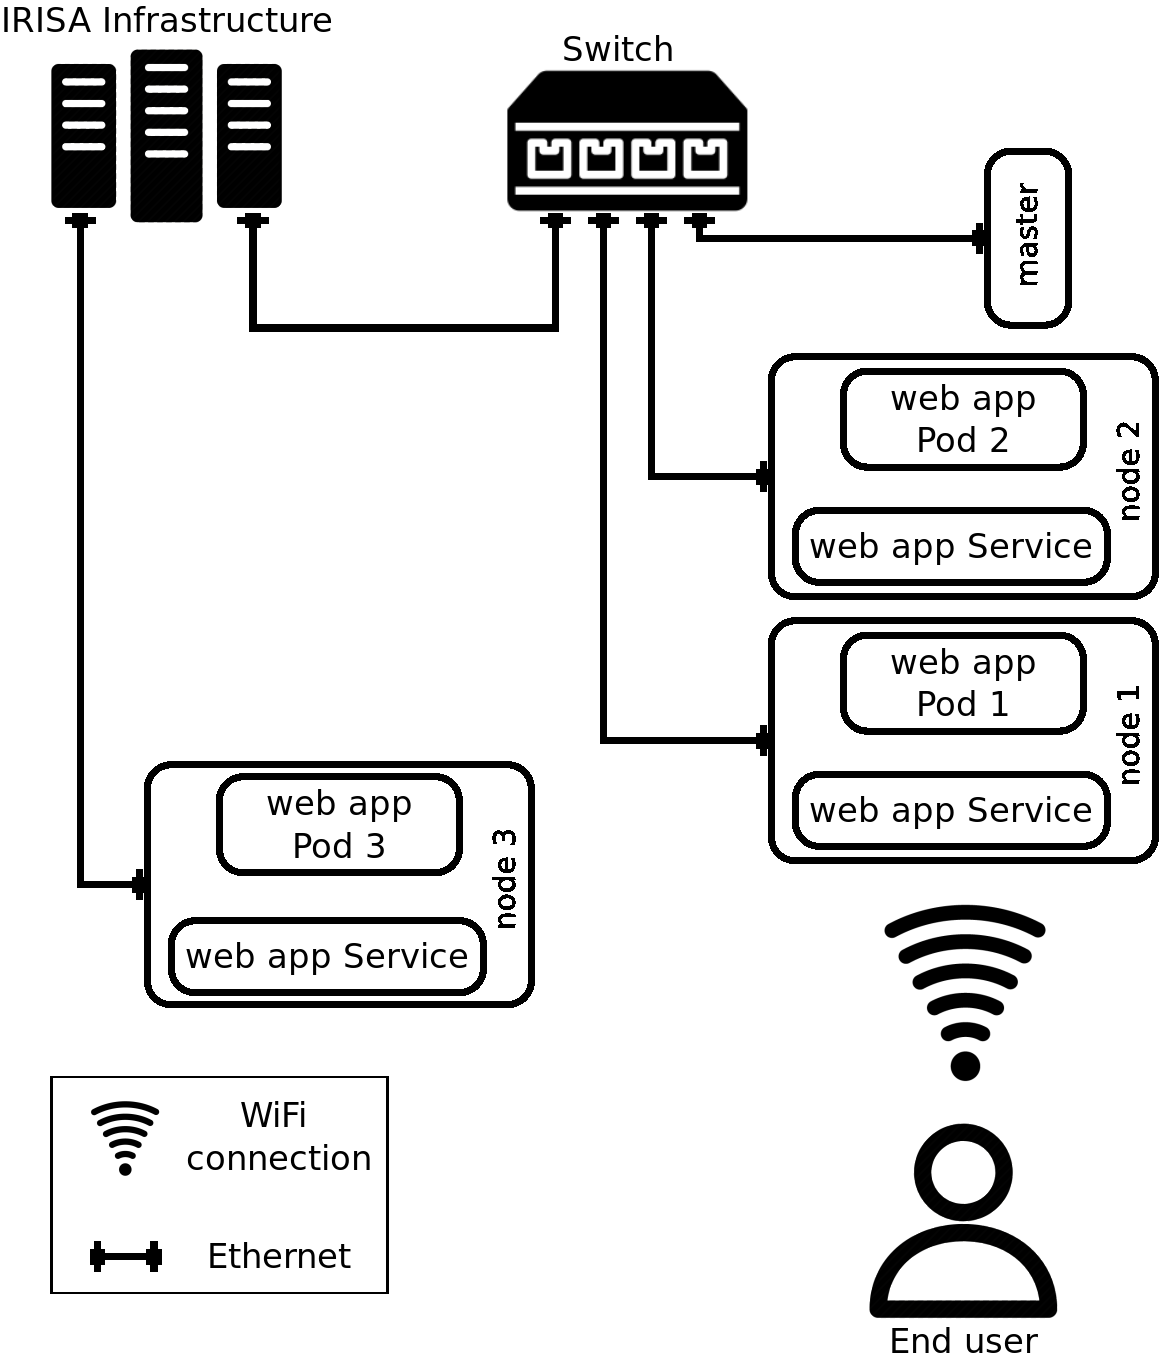
\includegraphics[width=0.4\textwidth]{images/clus.png}
\caption{Test topology}
\label{fig:clus}
\end{figure}
\begin{table}[h]
\begin{center}
\begin{tabular}{ c  c || c  c c}

& & \multicolumn{2}{c} {Node} & \\
& & node 1 & node 2 & \\
\hline 
\multirow{4}{1em}{\begin{turn}{90}Packet size \end{turn}} & 30 byte & 0.2 ms & 2.5 ms & \multirow{4}{1em}{\begin{turn}{90} Latency \end{turn}}\\
& 100 byte & tbd ms & tbd ms &\\
& 1000 byte & tbd ms & tbd ms &\\
& 50,000 byte & 0.37 ms & 16.9 ms &\\
\hline
& Network hops & 1  & 3 & 
 
\end{tabular}
\caption{Pods Performance as function of the selected pod}\label{tab:lat}
\end{center}
\end{table}

We have collected the latency for each of the pods over 1000 times, the latency was calculated by sending 50,000 byte UDP packets. To avoid overloading the pod we have separated the transmission of the packets by 1 second, preventing any delays caused by processing overhead. The result of these measurements are summarized in Table \ref{tab:lat}. Even in such an ideal conditions, where the nodes are connected using Ethernet cable and 100 Mbps switch and 1 Gbps switches in IRISA infrastructure. The results have reflected a significant increase of the latency between selecting the pod located in the node we are communicating with and any pod located elsewhere. 

The difference between a node located in the 

The absence of location awareness is not only needed while sending requests, but also at the deployment of the pods. Consider Figure \ref{fig:dep} where the mesh represents the geographical distribution of cluster consist of 40 nodes, with an application that have 4 replica pods. If the deployment container of k8's did not consider the location of the nodes, the replicas can be located in a problematic manner as in case 2, and vice-versa for case 1. \change{rephrase!}

\begin{figure}[th]
\centering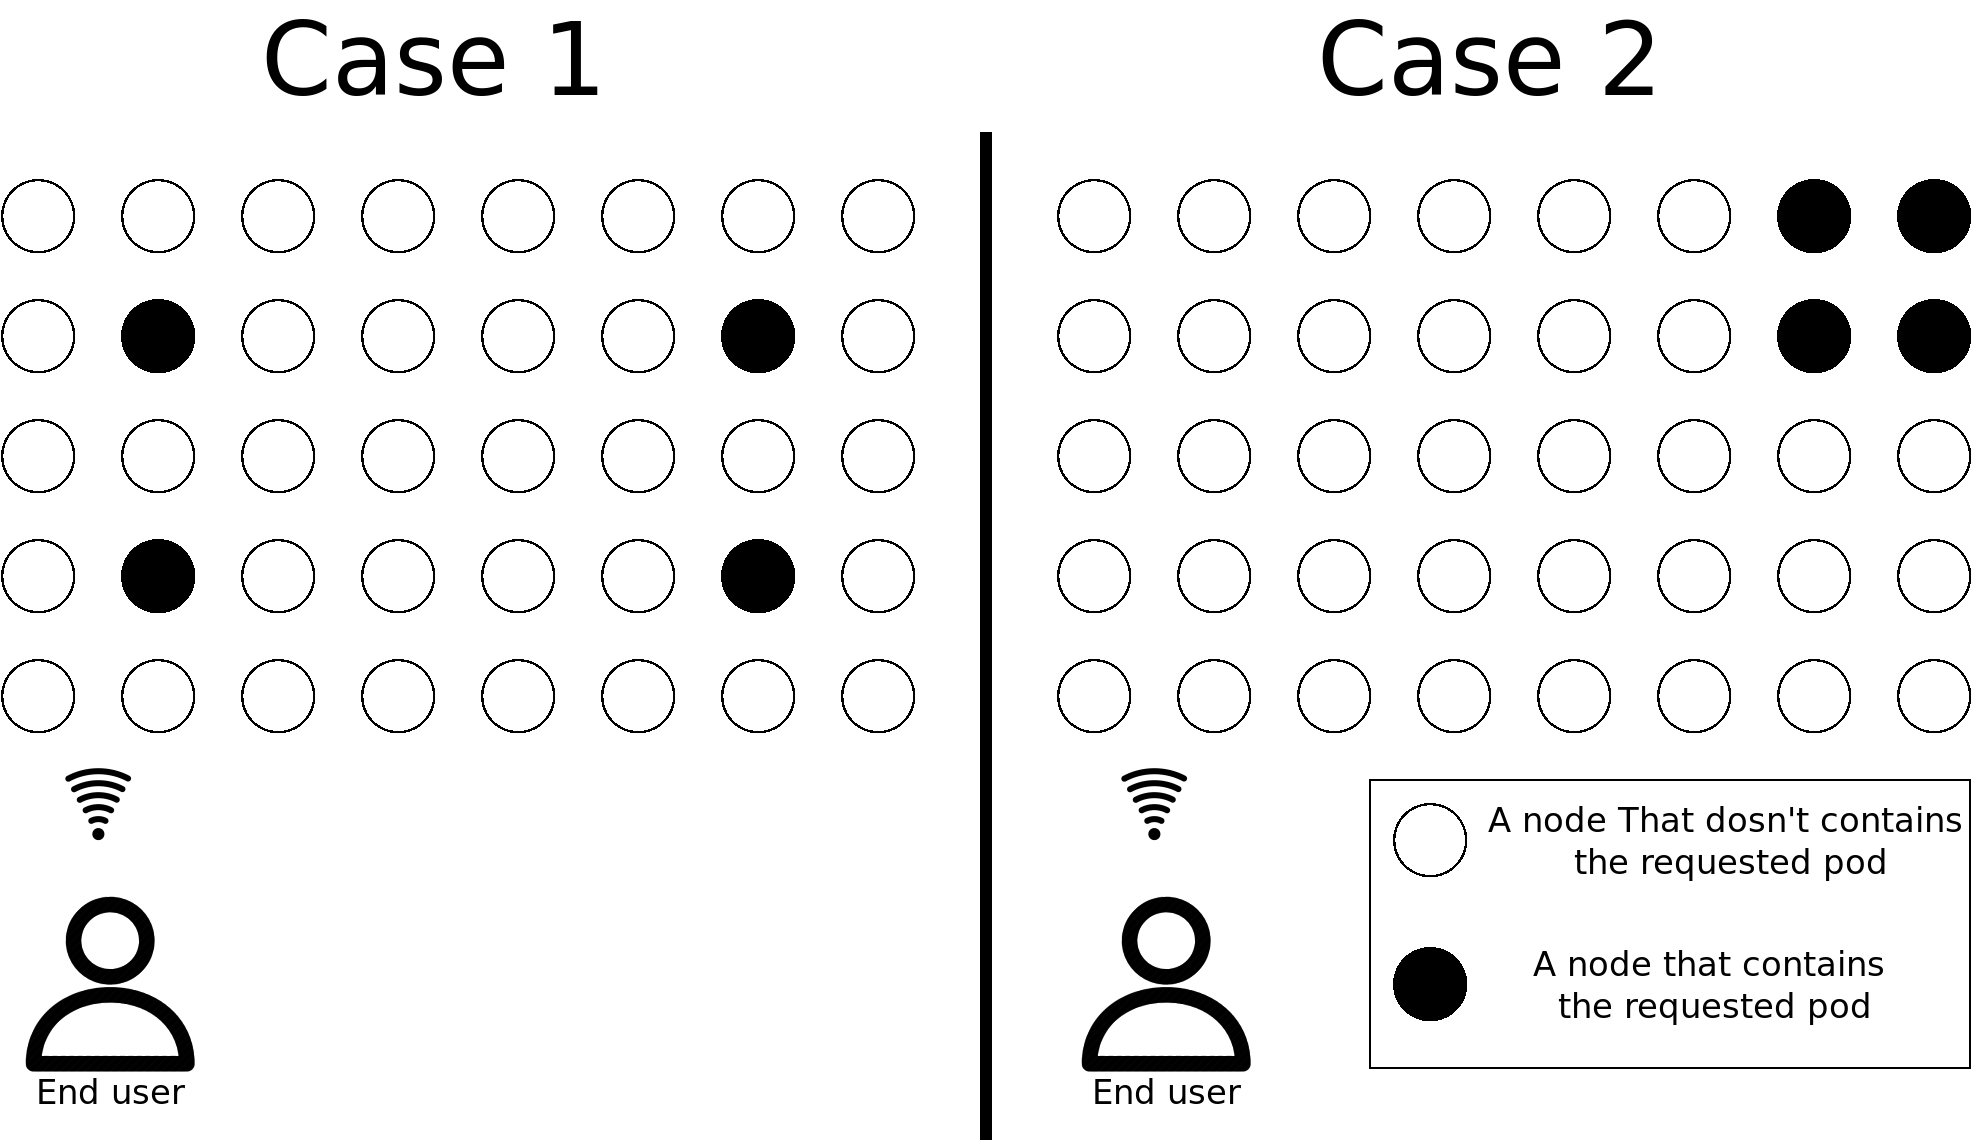
\includegraphics[width=.5\textwidth]{images/dep.png}
\caption{Pod deployments}
\label{fig:dep}
\end{figure}


The steps that have to be taken should include adding a new measure that describe the K8's nodes, this measure would give us the exact location of the node by using GPS for example, or this measure will give us a great estimation of the location.\unsure{what you think about the measure that have to be used!}. 
The second step toward location awareness is creating a new service type that will take the location of the node as a measure for the end user's jobs scheduling in addition of the load balancing alone.\change{add the code of the clusterIP}

Also the location should be considered in the deployment policy of the pods. Imagine a cluster that have 100 nodes, and the maintainer would like to implement an application that have 4 replications, the location of each of those pods is essential, since locating the four of them is the proximity of each others will induce higher latencies for the far nodes, the best solution would be locating them in a way that covers the 100 nodes as equally as possible. 

Both of the previously mention steps would need state-of-the-art algorithms that will take all the factors and available pods to choose the best pod to be used, still, starting from the simplest algorithms like choosing the closest node would be a good start before digging deep in more complicated algorithms.

%\subsection{Scheduler Decentralization}

%One of the disadvantages of Kubernetes as a fog platform is the centralization of the infrastructure, where the main components like the controllers and the scheduler are located exclusively in the master. which will impose higher latencies and heavy computations (at least for a Raspberry Pi). 

%The deployment of the pods are done in the following way: 
%\begin{itemize}
%\item The resource pool. 
%\item The scheduling. 
%\item the deployment.
%\end{itemize} 

%all of the previous components are centralized in our future work we will try to decentralize each of the components starting from the deployment controller. 
%where our long term goal is reaching a fully decentralized k8's. 





%%%%%%%%%%%%%%%%%%%%%%%%%%%%%%%%%%%%%%%%%%%%%%%%%%%%%%%%%%% Conclusion %%%%%%%%%%%%%%%%%%%%%%%%%%%%%%%%%%%%%%%%%%%%%%%%%%%
\section{Conclusion}\label{sec:conclusion}

In this paper, we have targeted the challenges the fog have nowadays,
the lack of a fully compatible platforms, and the need to add some key
elements to the currently available platforms. We have added the
motivation to update Kuberenetes to support the fog needs throughout
running our own cluster and tackling the main issues we face. Finally,
we have proposed our vision for the upcoming steps, that will be our
next objective.

%%%%%%%%%%%%%%%%%%%%%%%%%%%%%%%%%%%%%%%%%%%%%%%%%%%%%%%%%%% Acknowledgments %%%%%%%%%%%%%%%%%%%%%%%%%%%%%%%%%%%%%%%%%%%%%%%%%%%
% \section{Acknowledgments} 
% \change{keep it for the prof., I don't know whom exactly is paying me :p }
% \change{You are being paid by the Ministry of Higher Education and Research. They don't demand that we acknowledge them\ldots}



\theendnotes


{\footnotesize \bibliographystyle{acm}
\bibliography{fogaware}}
% \newpage
% \listoftodos[Notes]




\end{document}







